\section{Auswertung} \label{sec:auswertung}

\subsection{Modell} \label{subsec:modell}

Für die Berechnung der potentiellen Energie benützen wir das Modell Park Avenue 432, eines der höchsten reinen Wohnhochhäusern auf der Welt. Die stolze Höhe und der über das ganze Gebäude gleichbleibende quadratische Grundriss sind ideal für unsere Berechnungen. Für die Wassermengenberechnung stützen wir uns auf die Angaben des durchschnittlichen Wasserverbrauch in Amerika pro Person und Tag: 314\si{L}. \cite{waterUsAmerica}

\begin{figure} [H]
	\centering
	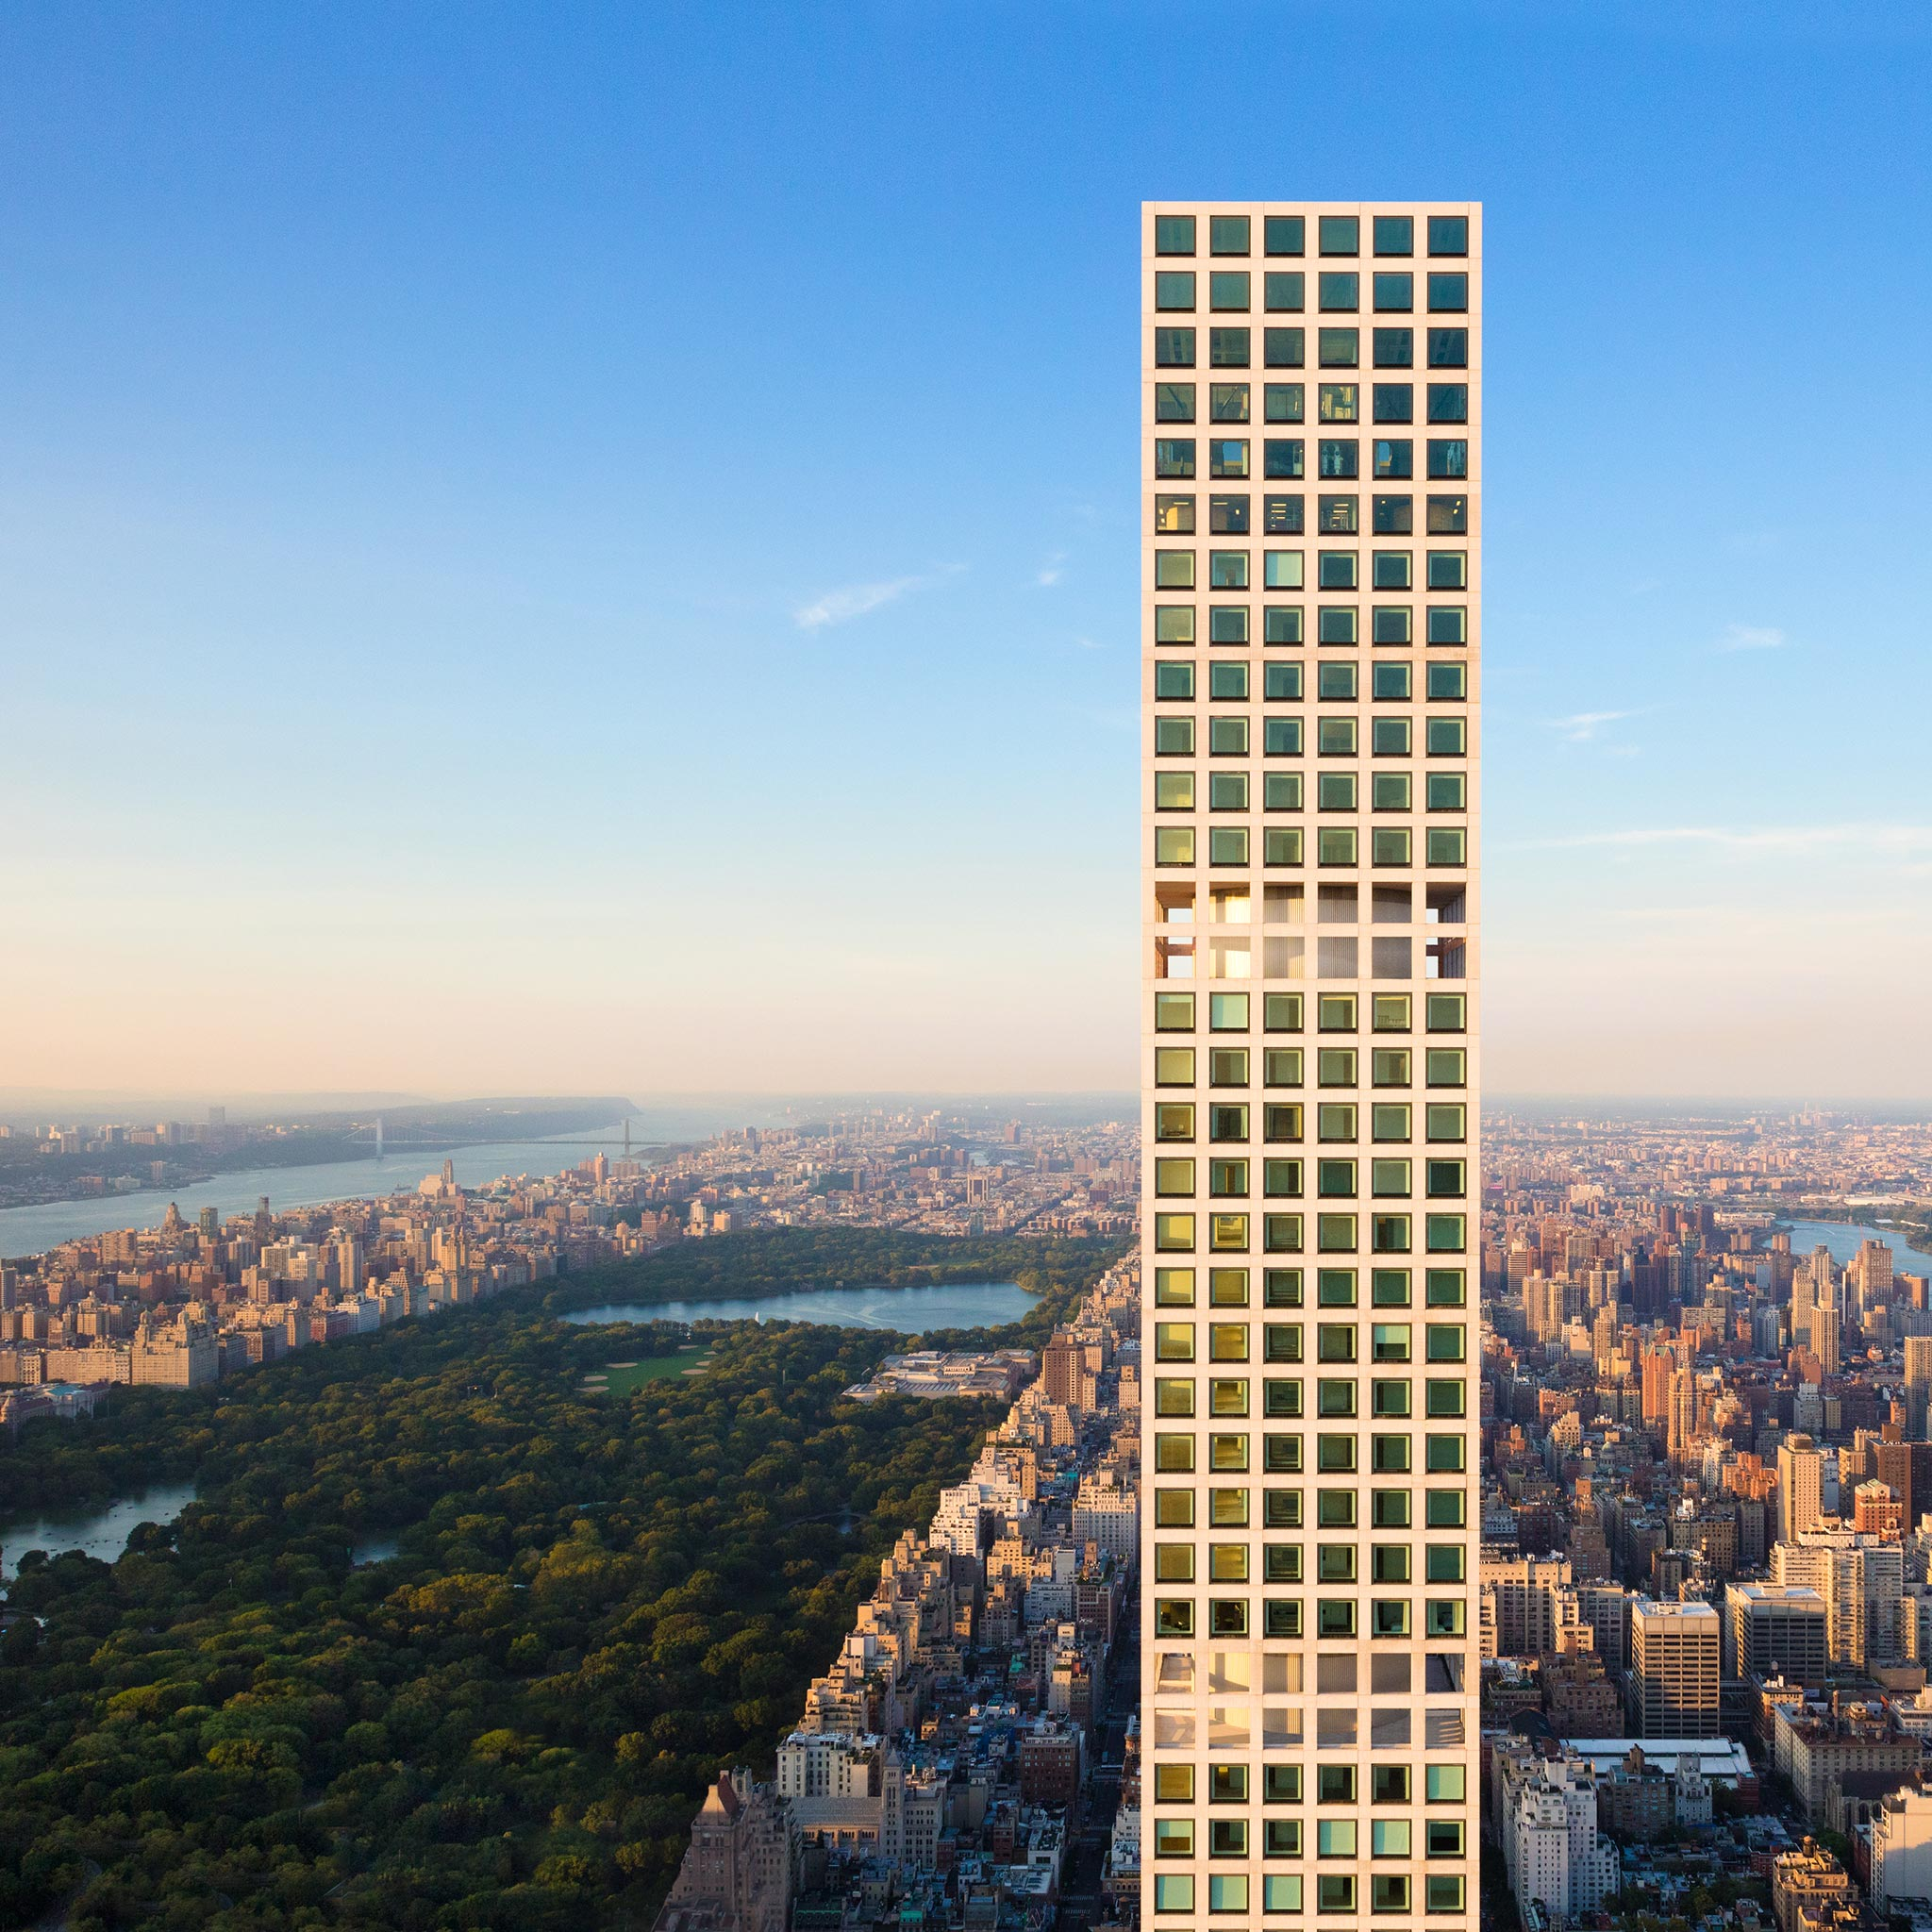
\includegraphics[width=12cm]{parkAvenue.jpg}
	\caption{Park Avenue 432 \cite{432_Park_Avenue}}
	\label{fig:Park_Avenue_432}
\end{figure}

\begin{table}[H]
\centering
\begin{tabular}{ll}
Name:				&Park Avenue 432\\
Höhe: 				&426m\\          
Etagen:				&84 Obergeschosse, 1 Erdgeschosse, 3 Untergeschosse\\
Etagenhöhe:			&4.72m\\
Hoechste Etage:		&392.1m\\
Wohnungen:			&146\\
Speziell:			&alle 12 Etagen 2 Etagen leer\\           
\end{tabular}
\end{table}

\newpage


\subsection{Energieberechnung} \label{subsec:energieberechnung}

Die Endgeschwindigkeit des Wassers kann mit folgender Formel berechnet werden:
\begin{center}
\(v = \sqrt{2 \cdot g \cdot h} \)
\end{center}

Die Einheit der Geschwindigkeit \(v\) ist \si{m/s}, das Schwerefeld \(g\) auf der Erde besitzt den Wert 9.81~\si{N/kg}, und die Höhe \(h\) hat die Einheit \si{m}.

\bigskip

Die Energie, die gewonnen werden kann, wird mit folgender Formel berrechnet:

\begin{center}
\(E =\frac 12\ \cdot m \cdot v^2\)
\end{center}

Die Energie \(E\) hat die Einheit \si{J}, die Einheit der Geschwindigkeit \(v\) ist \si{m/s}, und die Masse \(m\) hat die Einheit \si{kg}

\bigskip

Um die Leistung zu erhalten, muss die Masse pro Zeit(1s) einberechnet werden. Die Masse wird mit der Dichte und dem Volumenstrom ersetzt.

\begin{center}
\(P =\frac 12\ \cdot \varphi \cdot Q \cdot v^2\)
\end{center}

Die Leistung \(P\) hat die Einheit \si{W}, der Volumentstrom \(Q\) die Einheit \si{m^3/s}, die Dichte \(\varphi\) \si{kg/m^3} und die Geschwindigkeit \(v\) \si{m/s}.

\newpage

Mit diesen Mathematischen Grundlagen kann nun die Energie an unserem Modellhochhaus für beide Grobkonzepte berechnet werden. Für die Berchnungen wird angenommen das pro Wohnung 2.5 Personen leben und sie einen Durchschnittverbrauch pro Tag von 314\si{L} haben.

Bei 146 Wohnungen und 74 Nutzbaren Etagen leben 5 Personen pro Etage. Es wird somit 1570\si{L} pro Etage pro Tag verbraucht.

\bigskip

\paragraph{Grobkonzept 1} 



\paragraph{Grobkonzept 2}

Mit dem Grobkonzept 1 kommt man total auf ********. Mit dem Grobkonzept 2 kommt man total auf *******. Die Berechnungen sind im Anhang unter  ersichtlich \ref{subsec:grobkonzept1} \nameref{subsec:grobkonzept1} und \ref{subsec:grobkonzept2} \nameref{subsec:grobkonzept2} ersichtlich




\subsection{Kostenberechnung} \label{subsec:kostenberechnung}